\chapter{Konzeption} % Das würde eigentlich 'Konzeption' heißen aber Tichy wirkt stark in mir

In diesem Kapitel werden die Konzepte beschrieben, die die in \autoref{sec:novelty} 
beschriebenen Probleme untersuchen sollen. Hierfür bietet \autoref{sec:concept-overview}
\textit{\nameref{sec:concept-overview}}
zunächst eine Übersicht der in diesem Kapitel beschriebenen Inhalte, um das Vorgehen, 
die relevanten Neuerungen und deren Wichtigkeit für das Erfüllen der Ziele zu erkennen. 

\section{Übersicht} \label{sec:concept-overview}

\begin{figure}[h]
	\centering
	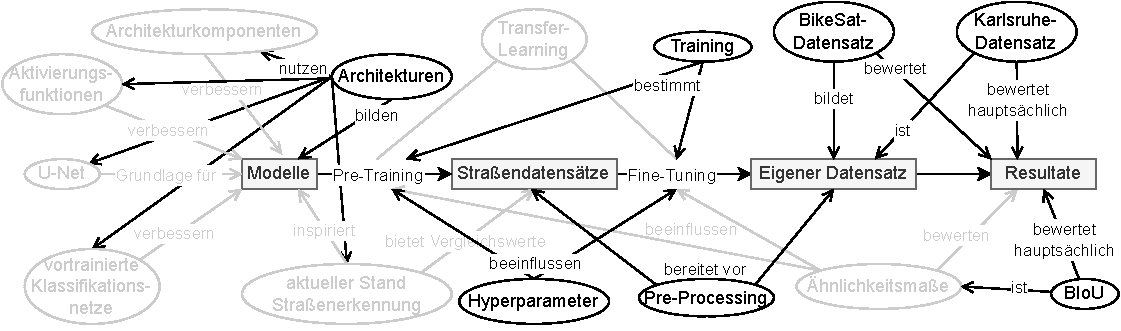
\includegraphics[width=1.\textwidth]{Bilder/overview.drawio.pdf} 
	\caption{Überblick über die relevanten Inhalte des Kapitels und wofür diese wichtig sind. Zentrale vier Kästen 
	beschreiben Hauptvorgehen in der Arbeit. Ausgegraute Elemente zeigen 
	Inhalte des Stands der Technik.}
	\label{fig:overview-concept}
\end{figure} 

\autoref{fig:overview-concept} zeigt eine Übersicht über die in diesem Kapitel relevanten Inhalte und wie diese 
zusammenspielen. Dabei nehmen die zentralen vier Kästen eine besondere Rolle ein: Sie beschreiben das grundsätzliche 
für diese Arbeit geplante Vorgehen, um zu einem guten Ergebnis für die Radwegerkennung zu gelangen. Das Vorgehen ist 
\autoref{sec:state-of-the-art-overview} beschrieben, grob sollen aber Modelle verschiedener Architekturen 
konzipiert werden, auf den Straßendatensätzen vortrainiert, dann auf einem neu zu erstellenden Datensatz für Radwegerkennung 
trainiert und schließlich untereinander verglichen werden, um die geeignetste Architektur und Methode des Trainings zu identifizieren. 
Die ausgegrauten Inhalte im Diagramm gehören zum Grundlagenkapitel, sind natürlich aber für die Konzeption relevant. \\ 
Wie in \autoref{sec:novelty} beschrieben, existiert kein Datensatz zur Erkennung von Radwegen. Daher wird hier 
der \textit{BikeSat}-Datensatz konzipiert, um zum Training verwendet zu werden. Weiter wird der \textit{Karlsruhe-Datensatz} 
erstellt, um die Ergebnisse auf einer anderen Stadt mit Bildern, die sich visuell vom BikeSat-Datensatz unterscheiden, zu testen. \\
Mit den eigenen Datensätzen kann dann eine geeignete Methode des Pre-Processing konzipiert werden, mit der die Datensätze 
auf das Training vorbereitet werden können. Wie in \autoref{sec:evaluation-metrics:quality} erwähnt, muss zudem 
eine geeignete Bewertungsfunktion für die Quantifizierung der Ergebnisse entwickelt werden, was in \autoref{sec:eval:biou} 
vorgenommen wird. Mit dem Wissen aus dem Grundlagenkapitel können die Architekturen für die zu vergleichenden Modelle entworfen werden 
und deren Hyperparameter festgelegt werden. Schließlich kann die Trainings- und Pre-Trainingsmethodik und die daraus resultierenden 
trainierten Modelle im Abschnitt \textit{Training} erörtert werden.  

\section{BikeSat-Datensatz} \label{sec:bike-data}

Da sich die im \autoref{sec:road-detection:roads-data} vorgestellten Datensätze zur Erkennung von Straßen nicht auf die Fahrradwege übertragen lassen, 
ist es erforderlich einen eigenen Datensatz, den \textit{BikeSat-Datensatz}, zu erstellen.
Prinzipiell gibt es die Möglichkeiten, die Datensätze manuell zu labeln oder automatisch generieren zu lassen.
Manuelles Labeln führt zu einer hohen Genauigkeit.
Allerdings ist diese Art der Datensatzerstellung entsprechend zeitintensiv und mit hohen Kosten verbunden.
Gerade lange Labelsessions sorgen für Ungenauigkeiten beim Einzeichnen der Ground Truth. 
In jedem Bild müssen Fahrradwege händisch erkannt werden, wobei die Wege nicht immer eindeutig als solche identifiziert werden können.\\
Für die Generierung der Labels müssen entsprechende Koordinaten bekannt sein, an denen sich Fahrradwege befinden.
Mithilfe dieser Punkte können dann Polygone in eine Maske eingezeichnet werden und erhält das zu einer Satellitenaufnahme zugehörige Bild.
Diese Art der Datensatzgenerierung ist deutlich weniger aufwändig als das manuelle Labeln. 
Ebenso können unter der Beschränkung der gegebenen Koordinaten und Satellitenbilder große Datensets erzeugt werden.
Abweichende Koordinaten wirken sich jedoch nachteilig auf die Qualität des Datensatzes aus, da keine menschliche Überprüfung im Anschluss erfolgt.
Aufgrund der Vielfältigkeit der Radwege, der damit verbundenen Größe des benötigten Datensatzes und dem geringeren Arbeitsaufwand, ist eine Entscheidung zugunsten der automatischen Datengenerierung gefallen.
Eine schlechtere Datenqualität des Labels wird hingenommen. \\
Die Abdeckung der automatischen Annotationen ist allerdings sehr gut. Auch wenn die 
automatisch generierten Label nicht immer die Position des Fahrradweges genau treffen, 
ist die Datengrundlage äußerst vollständig. Eine manuelle Sichtung der Datengrundlage mit 
einer Stichprobengröße von 234 zufällig 
ausgewählten Bildausschnitten, die laut Datengrundlage insgesamt 722 Radwege enthalten, hat ergeben, 
dass lediglich zwei Radwege nicht in der Datengrundlage verzeichnet sind. Es sind also \textbf{722} 
von \textbf{724} realen Radwegen in der Stichprobe enthalten. Demnach wird der Einfluss von 
fehlenden Radwegen auf das Training als eher gering eingestuft.   
 

\begin{figure}
	\centering
	\includegraphics[width=.6\textwidth]{Bilder/Hannover.png} 
	\caption{$2000{\times}2000~ m^2$ Luftaufnahmen-Ausschnitt von Hannover.}
	\label{fig:hannover-data}
\end{figure} 

Die Erstellung ist in mehreren Schritten vorgenommen worden.
Zunächst mussten Satellitenbilder unter Berücksichtigung der \ac{GSD} ausfindig gemacht werden.
In dem durch die Luftbilder abgedeckten Gebiet sind anschließend offizielle Fahrradwege aus einer API ausgelesen worden.
Mit den vorhandenen Informationen konnten dann die zugehörigen Masken gezeichnet werden.
In den nachfolgenden Unterkapiteln werden auf die Einzelschritte detaillierter eingegangen.

\subsection{Satellitenbilder}

Für die zu Satellitenbilder wird eine entsprechend niedrige \ac{GSD} von $20 \frac{cm}{px}$ benötigt, damit sich Radwege erkennen lassen. 
Aufgrund der aufwändigen Gewinnung und Aufbereitung der Orthofotos, sind diese meist nur kostenpflichtig zu erlangen.
Das Landesamt für Geoinformation und Landesvermessung Niedersachsen jedoch stellt Orthofotos in der benötigten Qualität kostenfrei zum Download zur Verfügung.
Der Datenbestand umfasst flächendeckend ganz Niedersachsen mit einer Aktualität von 3 Jahren.
Für die Datenset-Generierung ist ein Auszug der verfügbaren Städte verwendet worden, Hannover, Oldenburg, Osnabrück und Braunschweig. 
Der Download in diesem Bereich umfasst dann die Aufnahmen als je $2{\times}2 ~km^2$-Kacheln ($10.000{\times}10.000{\times}3$ Bilder)\cite{.26.10.2022}.
\autoref{fig:hannover-data} zeigt ein solches Bild. 
Für eine bessere Generalisierung des neuronalen Netzes, sind mehrere Städte verwendet worden.
Die jeweilige Anzahl der Aufnahmen pro Stadt lässt sich \autoref{tab:city-distribution} entnehmen.
Die Gesamtsumme beträgt 143 Satellitenbilder, also 572 $km^2$ Fläche.
Der benötigte Speicherplatz für den gesamten Datensatz beträgt $3,05 GB$.

\begin{table}
	\centering
	\begin{tabular}{l|l|l|l|l|l}
		& Hannover & Oldenburg & Osnabrück & Braunschweig & Summe\\
		\midrule
		Absolut & 72 & 21 & 20 & 30 & 143\\
		Anteil & $50,35$ & $14,68$ & $13,99$ & $20,98$ & 100 \\
	\end{tabular}
	\caption{Aufteilung der Satellitenaufnahmen auf die einzelnen Städte.}
	\label{tab:city-distribution}
\end{table}

Auch bei der Stadt Karlsruhe können Luftaufnahmen von Karlsruhe in benötigter Qualität für Lehre und Forschung kostenfrei beantragt werden.
Der Richtwert für die zu beantragende Größe beträgt $1km^2$.
Da in diesem kleinen Ausschnitt nicht genügend Fahrradwege enthalten sind, um ein neuronales Netz trainieren zu können, dienen diese Daten als Testdatensatz.
Mehr dazu in \autoref{sec:karlsruhe} \cite{.04.12.2022}.

\subsection{Auslesen der Fahrradwege} \label{subsec:overpass-api}

Eingetragene Radwege können über die Overpass API von \ac{OSM} ausgelesen werden \cites{.05.10.2021}{OpenStreetMapcontributors.2017}.
Innerhalb der Anfrage kann zwischen einer Vielzahl von Attributen unterschieden werden.
Alle Radwege und Fahrradstreifen innerhalb der angegebenen Zone sollen zurückgeliefert werden.
Auch einseitige Radwege werden ausgegeben. 
Die jeweiligen Attribute geben Aufschluss darüber, ob es sich um einen links- oder rechtsseitigen Weg handelt.
Der mitgegebene Bereich entspricht genau der Abdeckung durch die Satellitenbilder.
Die ausgelesenen Daten können als GeoJSON exportiert werden.
Bei Straßen werden Fahrradstreifen zentriert, statt seitlich an der korrekten Position zurückgegeben.
Dies muss nachher bei der Maskenerstellung entsprechend berücksichtigt werden. Die Anzahl der vorhandenen Fahrstreifen der Straße lässt sich ebenfalls aus den gelieferten Daten entnehmen.
Außerdem werden die Koordinaten für die Fahrradwege beispielsweise bei Kreuzungen oder Brücken durchgehend zurückgegeben. 
Hier lassen sich aus Satellitensicht keine Wege erkennen, was später zu Kosten für das Netz führt, obwohl sich keine Radwege erkennen lassen.
Über manuelles Labeln können diese Bereiche ausgespart werden können, was zu einer besseren Ground Truth führt, bzw. dem, was sich vom neuronalen Netz erwarten lässt.

\begin{figure}
	\centering
	\begin{minipage}{.45\textwidth}
		\centering
		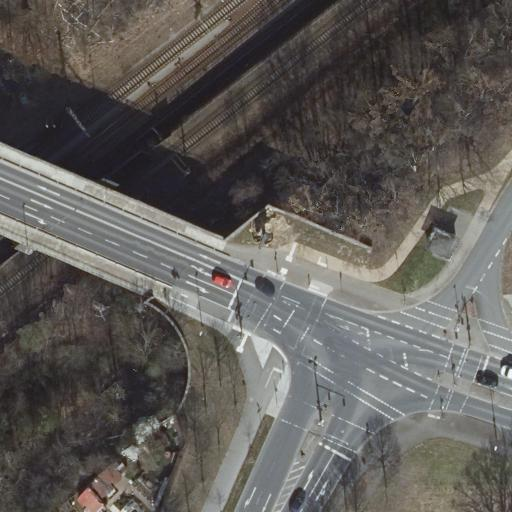
\includegraphics[width=.7\linewidth]{Bilder/good-cut-ex.png} 
	\end{minipage}
	\begin{minipage}{.45\textwidth}
		\centering
		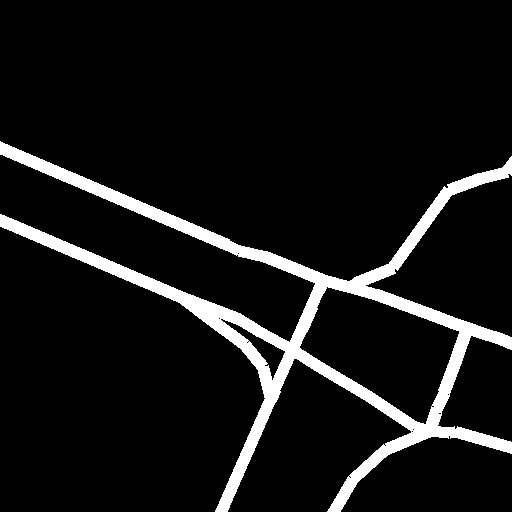
\includegraphics[width=.7\linewidth]{Bilder/good-cut-ex-mask.png} 
	\end{minipage}

	\caption{$512{\times}512$-Pixel-Auschnitt des BikeSat-Datensatzes (links) 
	mit zugehöriger optimal automatisch generierter Maske (rechts).}
	\label{fig:good-mask}
\end{figure} 

\subsection{Maskenerstellung}

Mit den vorhandenen Orthofotos und den Koordinaten der Radwege können nun die Masken generiert 
und deren Güte abgeschätzt (s. Ende des Unterabschnittes) werden.
Dafür werden zunächst die einzelnen Wege in zwei Klassen aufgeteilt, \textit{Fahrradwege} und \textit{Fahrradstreifen}.
Die zugehörigen Koordinaten werden als Liste mit Breiten- und Längengraden übergeben.
Für die in \autoref{subsec:overpass-api} erwähnte Verschiebung werden zusätzlich die Anzahl der Fahrspuren sowie die Existenz eines links- oder rechtsseitigen Weges berücksichtigt.
Die Berechnung wird heuristisch über die Anzahl an Autospuren durchgeführt.
Je mehr Spuren vorhanden sind, desto weiter muss der Fahrradstreifen verschoben werden.
Es wird die durchschnittliche Breite einer Fahrbahn von, also eine Verschiebung um, $17.625px$ angenommen.
Fahrradwege werden hingegen nicht verschoben, da diese passend von Menschen annotiert sind.\\
Für jedes Satellitenbild wird zunächst eine leere Maske erstellt.
Mithilfe der Koordinaten, die bei den einzelnen Klassen gespeichert sind, können die Linien eingezeichnet werden.
Dafür werden die Koordinaten auf die korrespondierenden Pixelkoordinaten transformiert.
Die Breite der einzuzeichnenden Linien orientiert sich an dem Durchschnitt verschiedener Radwege, welcher sich auf $11,8125px$ beläuft.
\autoref{fig:good-mask} zeigt einen Luftbildausschnitt (links) zusammen mit der dafür automatisch generierten Maske (rechts),
wobei die automatische Annotation sehr gut funktioniert. 

\subsubsection{Güteabschätzung der Masken}

\begin{wrapfigure}{r}{0.40\textwidth}
	\centering
	\vspace{-30pt} % Manchmal möchte man den oberen Abstand selbst anpassen
	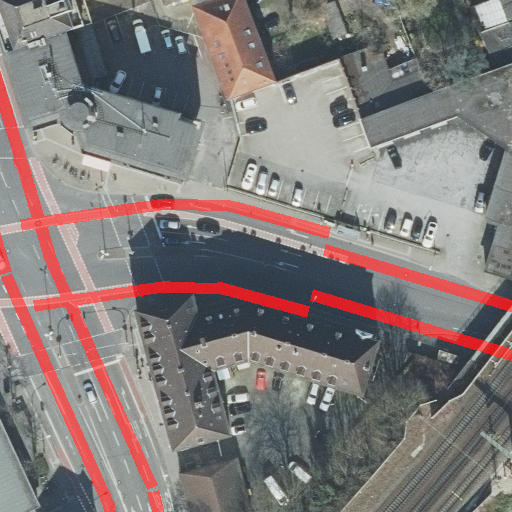
\includegraphics[width=0.35\textwidth]{Bilder/bad-mask-example.png}
	\vspace{-10pt}
	% Das folgende ist ein Trick, um "Abbilgung x.y" in eine
	% eigene Zeile zu packen. Der Text zwischen [ und ] steht
	% im Abbildungsverzeichnis. Der Text darunter wird
	% tatsächlich angezeigt.
	\caption[Schlechte Maske eines $512{\times}512$-Ausschnittes aus BikeSat-Datensatz.]{\unskip}
	$512{\times}512$-Ausschnitt aus BikeSat-Datensatz mit rot-überlagerter, mangelhaft automatisch generierter Maske.
	\label{fig:bad-mask}
\end{wrapfigure}

Die Heuristik beim Einzeichnen der Maske führt dazu, dass manchmal Radweg in Grünstreifen oder auf Straßen eingezeichnet werden, da sie falsch verschoben worden sind.
\autoref{fig:bad-mask} zeigt ein solches Negativbeispiel: Großteil der Annotationen (heuristisch generiert) trifft den eigentlichen Radweg nicht. 
In der Straßenmitte befindliche Schienen für Straßenbahnen werden ebenfalls nicht berücksichtigt.
Beim Übergang zwischen Fahrradstreifen und -wegen kommt es häufig zu einer sprunghaften Veränderung, die es dem neuronalen Netz erschweren, durchgängige Linien einzuzeichnen.
Die geschätzte Pixelbreite eines Weges stimmt nicht immer exakt überein, bietet aber einen relativ zuverlässigen Ausgangspunkt, wegen geringerer Varianz in den Stichproben, 
die zur Ermittlung erhoben sind.

Das Problem bei den generierten Masken sind nicht die Fahrrad\textit{wege}, denn diese sind von Menschen manuell annotiert und damit passend im Satellitenbild, 
sondern die Fahrrad\textit{streifen}, denn diese sind durch die Heuristik ggf. daneben oder enthalten die beschriebenen Sprünge. \\
Der Anteil an manuell annotierten Fahrradwegen und heuristisch annotierten Fahrradstreifen kann Aufschluss über die Güte geben. 
Dieser Anteil trifft aber noch keine Aussage über die Länge der jeweiligen Wege. Um dies zu berücksichtigen, werden stattdessen die Kanten die zu 
entweder Fahrradwegen oder Fahrradstreifen gehört gezählt. Hier liegt die Annahme zugrunde, dass Kanten im Schnitt ähnlich lang sind.\\
Im Datensatz gibt es $129205$ Kanten die zu manuell annotierten Fahrradwegen gehören und $53256$ Kanten die zu heuristisch annotierten Fahrradstreifen gehören. 
Demzufolge sind ungefähr $70,8\%$ der Daten manuell und circa $29,2\%$ der Daten heuristisch annotiert. 
Aus Stichproben der heuristisch annotierten Fahrradstreifen lässt sich abschätzen, dass circa $30\%$ der Fahrradstreifen falsch liegen 
(kaum bis wenig Überschneidung mit dem Fahrradweg; $<30\%$ Überschneidung), circa $50\%$ grob richtig liegen (ungefähr $50\%$ Überschneidung)
und $20\%$ komplett richtig ($>80$ Überschneidung) liegen. Wird für grobe Richtigkeit ein Faktor von $\frac{1}{2}$ angenommen, so sind insgesamt
als Gütemaß $0,292 \cdot (0,3 + \frac{1}{2} \cdot 0,5) = 0,1606$ also $16,06\%$ der Annotationen falsch, bzw. 
\textbf{83,94\%} des Datensatzes auf dem Niveau einer manuellen Annotation. 
   
% dafür kannst du natürlich viele Bilder in das Kapitel ballern
% der datensatz-code hat jetzt auch die möglichkeit den ganzen karren mit rotem overlay von radwegen zu generieren

\section{Karlsruhe-Testdatensatz} \label{sec:karlsruhe}


\begin{figure}[h]
	\centering
	\includegraphics[width=0.6\textwidth]{Bilder/karlsruhe-data-shrinked.png} 
	\caption{Karlsruhe-Datensatz: $1433{\times}1433~ m^2$ Luftaufnahmen mit Radstreifen cyanfarben annotiert.}
	\label{fig:karlsruhe-data}
\end{figure} 

Der Karlsruhe-Datensatz besteht aus Luftaufnahmen und manuell von Menschen annotierten Masken von Fahrradstreifen 
über eine Stadtfläche von $1433{\times}1433~ m^2$ bzw. ca. $2,054~ km^2$, was im Vergleich zu den 
$572~ km^2$ des BikeSat-Datensatzes also eher wenig ist. Ein Pixel im Karlsruhe-Datensatz entspricht $0,2~m$, 
also hat der Datensatz eine GSD von $20 \frac{cm}{px}$.
Der gesamte Datensatz samt rot annotierter Radstreifen ist in einem 
$7168{\times}7168$ Pixel großen Bild in \autoref{fig:karlsruhe-data} zu sehen. Es fällt auf, 
dass nur die drei großen Straßen Radstreifen enthalten. Das Luftbild zeigt einen Ausschnitt der Karlsruher Weststadt im März 2022. 


Aufgrund der geringen Größe des Datensatzes wird dieser lediglich zum Testen der trainierten Modelle verwendet. 
Da es sich um eine andere Stadt handelt und die Bilder visuell anders geartet sind, als aus dem BikeSat-Datensatz 
kann dieser Datensatz die Generalisierungsfähigkeit des Netzes gut testen, insbesondere, da der Datensatz weder 
im Training noch in der Validation des BikeSat-Datensatzes vorkommt, wodurch es sich um wahrhaftig neue Eingabedaten für die Modedelle handelt. 
Es ist auch vorteilhaft, dass im Datensatz Radwege eher unterrepräsentiert sind, womit getestet werden kann, 
ob Straßen allgemein alle Radwege erhalten oder eine echte Unterscheidung der Straßen im Modell stattfindet.


\section{Pre-Processing} \label{sec:pre-processing}

Dieser Abschnitt befasst sich mit dem Pre-Processing, welches auf den in \autoref{sec:bike-data} 
beschriebenen Datensatz angewandt wird. Insbesondere ist die Klassenimbalance, Eingabegröße, 
Training-Validation-Test-Split und die Daten-Augmentation zu diskutieren. \\
Für die Verwendung im Modell werden die Pixelwerte aller Bilder von $[0; 255] \subset \mathbb{N}$
auf $[0;1] \subset \mathbb{R}$ abgebildet, indem alle Kanäle - bei RBG drei, bei den Graustufen-Masken einer - durch 255 geteilt werden.
Dies vermindert die betragsmäßige Größe der Eingaben und aufgrund der Masken auch Ausgaben. 

\subsection{Eingabegröße und Klassenimbalanceausgleich}

Durch die semantische Segmentierung besteht bei der Erkennung der Fahrradwege eine starke 
Klassenimbalance zwischen den Radweg-Pixeln und den Hintergrundpixeln. Diese Klassenimbalance ist bei der Radwegerkennung drastischer 
als bei der Straßenerkennung, da auf einem Bild, auf dem ein Radweg zu sehen ist, 
tendenziell der Radweg sehr viel weniger Platz auf dem Bild einnimmt, als sonstige Strukturen, wie Vegetation, Gebäude und Straßen. 
Durch die automatische Generierung des Radweg-Datensatzes sind zudem viele Bilder von kleinen Orten,
Industriegebieten, Feldern und Wäldern vorhanden, die keinerlei eingezeichnete Radwege enthalten. 
Selbst in Bildern der Innenstadt haben oft nur größere Straßen dedizierte Radwege, während der 
Großteil des Bildes mit Wohngebiet gefüllt ist. 
Somit ist nur ein verschwindender Anteil aller Pixel des Datensatzes als Radweg markiert. 

\begin{wrapfigure}{r}{0.40\textwidth}
	\centering
	\vspace{-30pt} % Manchmal möchte man den oberen Abstand selbst anpassen
	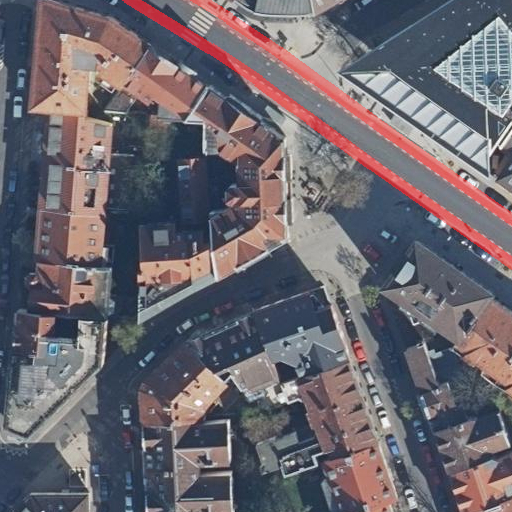
\includegraphics[width=0.35\textwidth]{Bilder/cut-example.jpg}
	\vspace{-10pt}
	% Das folgende ist ein Trick, um "Abbilgung x.y" in eine
	% eigene Zeile zu packen. Der Text zwischen [ und ] steht
	% im Abbildungsverzeichnis. Der Text darunter wird
	% tatsächlich angezeigt.
	\caption[Beispiel $512{\times}512$-Ausschnitt aus BikeSat-Datensatz.]{\unskip}
	Beispiel $512{\times}512$-Ausschnitt aus BikeSat-Datensatz mit roter Maske.
	\label{fig:cut-example}
\end{wrapfigure}

Um den Anteil an als Radweg annotierte Pixel zu erhöhen, sollen nur Bilder zum Training verwendet werden,
die überhaupt Radwege enthalten. Da es technisch zu ressourcenintensiv ist ein ganzes 
$10.000{\times}10.000$-Pixel-Bild einzugeben, sollen die Bilder in kleinere Stücke zerteilt werden. 
Dies ist auch bei den Modellen zur Straßenerkennung aus \autoref{sec:state-of-the-art-roads} die Praxis. 
Vorgeschlagene Ausschnittsgrößen können hierbei $256{\times}256$, $512{\times}512$ und $1024{\times}1024$ sein. 
Wird ein größerer Ausschnitt gewählt, steigt die Klassenimbalance, da häufig viele überflüssige 
Hintergrundpixel eingeschlossen werden, allerdings kein weiterer Radweg im Bild liegt. 
Wird eine kleine Größe gewählt, kann es sein, dass nur noch Radwege im Bild vorhanden sind, 
wodurch die Gefahr besteht, dass jede beliebige Straße einen Radweg seitlich angezeichnet bekommt. 
In kleinen Ausschnitten sind hauptsächlich stark ausgebaute Straßen mit Radwegen vorhanden. 
Schmalere und weniger gut ausgebaute Straßen sind aufgrund von fehlenden Radwegen kaum vorhanden, wodurch diese nicht als wahr-negativ gelernt werden.  
Außerdem tritt es bei kleinen Ausschnitten häufiger auf, dass Radwege nur sehr klein in den Ecken des Bildausschnittes
vorkommen und die lange zusammenhängende Struktur, die zu einem Radweg gehört, schwierige zu erlernen ist. 
Aus diesen Gründen wird als Kompromiss die $512{\times}512$-Größe gewählt. Somit entspricht eine Bildkante 
$512 \cdot 0,2m = 102,4m$. Die Zweierpotenz wird gewählt, 
sodass das Bild nicht zu klein wird in der U-Net-Struktur, bzw. damit eine saubere Teilung der 
Max-Pool-Schichten möglich ist, die die Bildkantenlängen stets halbieren. 

Jedes $10.000{\times}10.000$-Pixel-Bild und die dazugehörige Maske wird -- um den gesamten Bildinhalt zu erhalten -- in \textit{auf}gerundet
$\left\lceil{\frac{10.000}{512}}\right\rceil^2 = 400$ Teile geschnitten. 
Die aufgerundeten 39 Ausschnitte, die nur partiell im Bild liegen, werden im überstehenden Bereich mit Schwarz ($RGB=(0,0,0)$) gefüllt.
Damit ergeben sich bei 143 Bildern $143 \cdot 400 = 57.200$ $512{\times}512$-Bildausschnitte für den BikeSat-Datensatz. 
Der Karlsruhe-Datensatz lässt sich in ${\frac{10.000}{512}}^2 = 196$ Bildausschnitte teilen.\\
Weiter werden alle Ausschnitte entfernt, die keine oder fast keine als Radweg annotierten Pixel beinhalten. 
Die Quote wird auf 1\% festgelegt. Sollte also ein Bildausschnitt weniger als 1\% Fahrradweg-Pixel beinhalten, 
wird es entfernt. Durch diese Maßnahme sinkt die Anzahl an Bildausschnitten von $57.200$ auf $10.181$ Bildausschnitte - 
dieser Anteil entspricht ca. 17,7\%. Dieser Schritt wird für den Karlsruhe-Datensatz nicht durchgeführt. Hier bleiben alle 196 
Bildausschnitte erhalten.
 
\autoref{fig:cut-example} zeigt beispielhaft ein auf $512{\times}512$ Pixel zugeschnittenes Bild aus dem BikeSat-Datensatz 
mit der dazugehörigen Maske, die mit 50\% Transparenz in rot überlagert ist. Es ist zu erkennen, 
dass die Klassenimbalance noch recht stark ist, allerdings deutlich geringer, als in den ursprünglichen Bildern,
und dass auch trotzdem genügend Straßen ohne Radwege vorhanden sind und die Struktur und der Verlauf des Radweges 
bei der gewählten Ausschnittgröße weiterhin gut zu erkennen ist. 

\subsection{Training-Validation-Test-Split}

Zunächst werden die zerschnittenen Bilder aller Städte gemischt. Dann werden diese Ausschnitte disjunkt in 
Training-, Validation- und Test-Daten aufgeteilt. 
Damit sollten die unterschiedlichen Städte gleichermaßen in allen Teil-Datensätzen auftauchen, 
sodass der Test- und Validationdatensatz gut die Generalisierungsfähigkeit des Netzes überprüft. 
Durch die bereits höhere Zahl an Bildausschnitten (10.181 Stück) ist es eher unwahrscheinlich, 
dass eine ungleiche Verteilung der Städte vorkommt. Außerdem ist das Mischen wichtig, 
damit die Randausschnitte, die große schwarze Flächen beinhalten, anteilig gleich in 
jedem Teildatensatz repräsentiert sind, damit dies das Ergebnis nicht verfälscht, falls diese 
zum Beispiel nur in dem Validation- oder Testdatensatz vorkommen. 

\autoref{tab:bike-split} zeigt den im Folgenden verwendeten Trainings-Validation-Test-Split. 
Hierbei sind zwei Dinge zu bemerken, die nicht aus der Tabelle hervorgehen: 
Zunächst wurde der Testdatensatz abgespalten. Hierzu wurden 15\% vom Hannover-Datensatz und 
20\% von den jeweiligen Datensätzen der restlichen Städte als Testdatensatz abgespaltet. Da der Hannover-Datensatz so groß ist, wie die Datensätze der
restlichen Städte zusammen, läuft dies auf einen eher unkonventionellen Split von 17,5\% Testdaten hinaus. Diese Verteilung wurde so getroffen, 
um den Hannover-Datensatz etwas weniger zu gewichten, um im Test die Generalisierungsfähigkeit besser testen zu können
und den Einfluss der kleineren Städte auf die Generalisierungsfähigkeit zu erhöhen. Der Validation-Teildatensatz wurde danach aus 8\%, 
bzw. der Trainingsdatensatz aus 92\% vom Rest gebildet. \\
Der Trainingsdatensatz ist mit ca. 75\% der gesamten Daten eher groß gewählt, während der Validation-Datensatz eher klein gewählt ist. 
Nun kann ein größerer Validation-Datensatz dazu beitragen, die Hyperparameter besser zu optimieren. Das soll allerdings nicht Fokus der Arbeit sein.
Diese Entscheidung des großen Trainingsdatensatzes wurde getroffen,
um möglichst viele und unterschiedliche Bilder zum Training zu verwenden, da der Datensatz mit automatischer Synthese 
generiert wurde und daher qualitativ eher unvorteilhaft ist, wodurch eine höhere Anzahl an Trainingsdaten nötig wird.

\begin{table}
	\centering
	\begin{tabular}{l|l|l|l|l}
		& Training & Val. & Test & Summe \\
		\midrule
		Absolut & 7738 & 672 & 1771 & 10181 \\
		Anteil & 75,9 & 6,6 & 17,5 & 100 \\ 
	\end{tabular}
	\caption{Training-Validation-Test-Split des BikeSat-Datensatzes in gefilterten $512{\times}512$-Ausschnitten.}
	\label{tab:bike-split}
\end{table}


\subsection{Augmentation}

Die Bild-Augmentation wird nicht vor dem Training angewandt, um den Datensatz künstlich zu vergrößern, 
sondern während dem Training pseudo-zufällig mit festem Seed, um die Ergebnisse reproduzieren zu können.
Somit wird jedes Bild während des Trainings, bevor es in das Netz eingegeben wird zufällig augmentiert 
und dann eingegeben. Damit erhält ein und dasselbe Bild über die verschiedenen Epochen jedes Mal unterschiedliche 
Anpassungen auf Basis des Zufallsgenerators. Dies erhöht die Generalisierungsfähigkeit bzw. 
verringert die Gefahr von Overfitting. Das Netz sieht so viel mehr Varianten der Bilder. 
Nachteil ist, dass das Training länger dauert, da jedes Bild vor Eingabe bearbeitet wird. 
Dieser Nachteil ist vor allem evident, wenn mehrere Netze auf demselben Datensatz trainiert werden, da jedes Mal 
dieselben Augmentationen (da gleicher Seed) erneut vorgenommen werden müssen. Dieses Problem kann
durch eine Vorausberechnung der aufeinanderfolgenden Augmentationen behoben werden, worauf allerdings verzichtet wird,
da die Vorausberechnung parallel stattfinden kann. Ergebnisse zu den Laufzeiten sind im Ergebniskapitel zu finden. 

\begin{figure}
	\centering
	\begin{subfigure}{.32\textwidth}
		\centering
		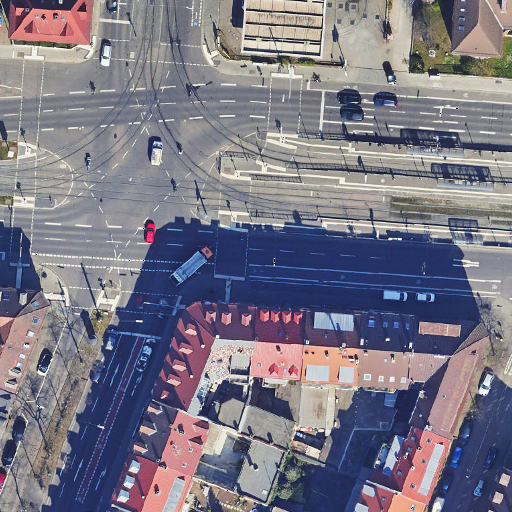
\includegraphics[width=1.\linewidth]{Bilder/color_aug/149_karlsruhe.png}
		Original
	\end{subfigure}
	\begin{subfigure}{.32\textwidth}
		\centering
		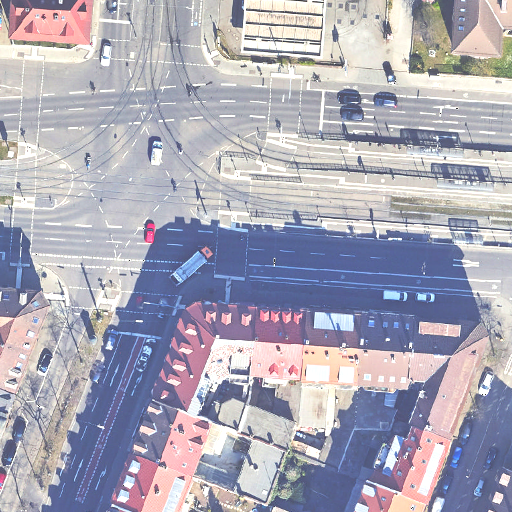
\includegraphics[width=1.\linewidth]{Bilder/color_aug/RandomBrightness.png}
		Helligkeit
	\end{subfigure} 
	\begin{subfigure}{.32\textwidth}
		\centering
		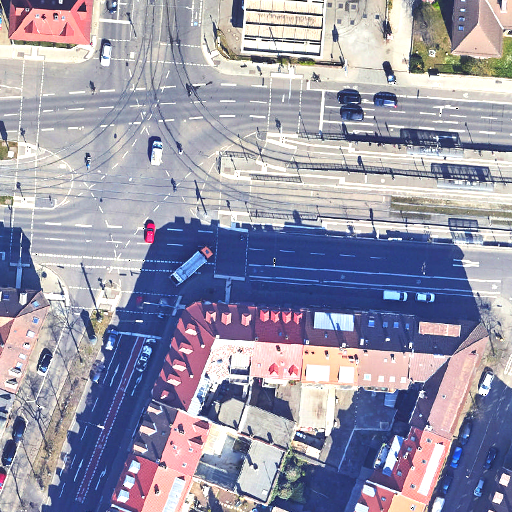
\includegraphics[width=1.\linewidth]{Bilder/color_aug/RandomContrast.png}
		Kontrast
	\end{subfigure} 
	\begin{subfigure}{.32\textwidth}
		\centering
		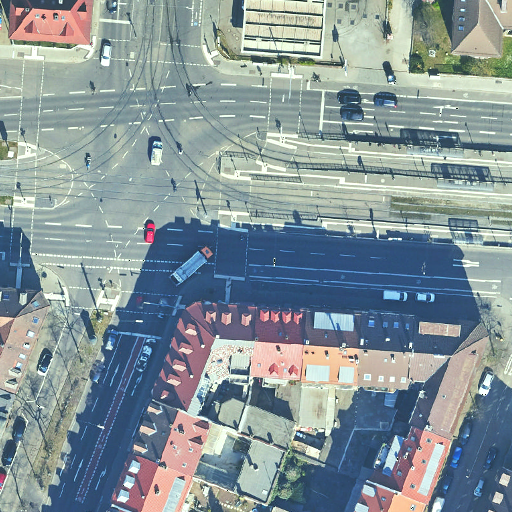
\includegraphics[width=1.\linewidth]{Bilder/color_aug/RGBShift.png}
		RGB-Shift
	\end{subfigure}
	\begin{subfigure}{.32\textwidth}
		\centering
		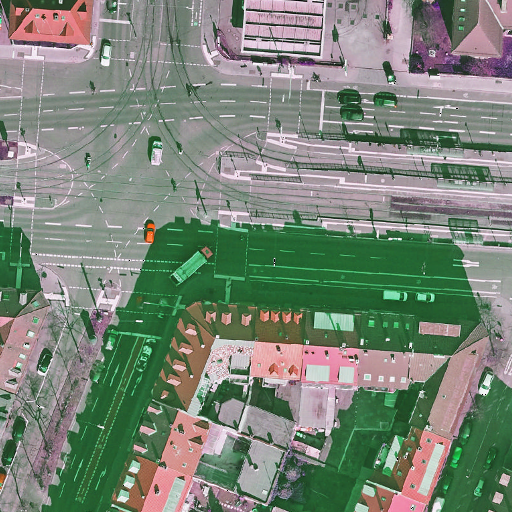
\includegraphics[width=1.\linewidth]{Bilder/color_aug/ChannelShuffle.png}
		Kanaltausch
	\end{subfigure}
	\begin{subfigure}{.32\textwidth}
		\centering
		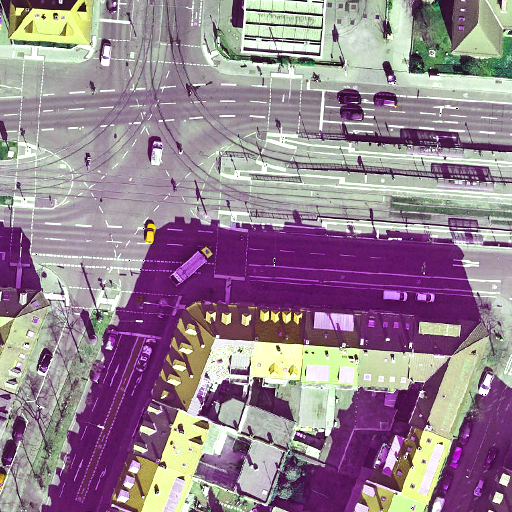
\includegraphics[width=1.\linewidth]{Bilder/color_aug/ColorJitter.png}
		Farb-Jitter
	\end{subfigure} 

	\caption{Beispielhafte Farb-Augmentierungen eines Beispielbildes mit Originalbild links oben. }
	\label{fig:color-aug}
\end{figure}

Jede der folgenden Augmentationen, wie beispielhaft zu sehen in \autoref{fig:augmentation} und \autoref{fig:color-aug}, 
werden in ihrem Wertebereich pseudo-zufällig angewandt. 
Sollte es die Veränderung erfordern, werden fehlende Bildteile mit Schwarz gefüllt. Schwarz wurde ausgewählt, da es ohnehin Bilder mit 
schwarzen Rändern im Datensatz gibt, weswegen das Netz hierbei mit nichts Neuem konfrontiert ist. 
\begin{enumerate}
	\item Rotation im Intervall von $[-90^\circ ; 90^\circ ]$. Eine Gradzahl wird für jedes Bild zufällig ausgewählt und angewandt. 
	Die dabei entstehenden leeren Bildbereiche werden mit Schwarz ($RGB = (0,0,0)$) gefüllt. 
	Diese Augmentation ist realistisch und nützlich, da Straßen in beliebiger Ausrichtung vorkommen und 
	eine natürliche Orientierung bei Bildern aus der Vogelperspektive nicht besteht.
	\item Horizontale Spiegelung. Es wird zufällig entschieden, ob ein Bild an der vertikalen Spiegelachse gespiegelt wird. 
	Diese Augmentation ist ebenfalls realistisch und hat gegenüber der Rotation den Vorteil keine schwarzen Flächen 
	einzuführen aber den Nachteil, nicht so viele neue Bilder erzeugen zu können. 
	\item Vertikale Spiegelung. Funktioniert wie die horizontale Spiegelung, allerdings wird an der horizontalen Achse gespiegelt. 
	Beide Spiegelungen können simultan auftreten, es gibt also vier Spiegelungs-Permutationen, 
	die mit gleicher Wahrscheinlichkeit auftreten.
	\item Horizontale Verschiebung im Intervall von $[-0,1 \cdot w; 0,1 \cdot w]$ Pixel entlang der horizontalen Achse,
	wobei $w$ die Breite des Bildes ist. Es wird eine zufällige Länge aus dem Intervall ausgewählt und verschoben; die 
	entstehenden Ränder werden mit Schwarz gefüllt. Auch diese Augmentation ist realistisch und erhöht lediglich 
	die Möglichkeit der Veränderung der Bilder. 
	\item Vertikale Verschiebung im Intervall von $[-0,1 \cdot h; 0,1 \cdot h]$ Pixel entlang der vertikalen Achse,
	wobei $h$ die Höhe des Bildes ist. Ansonsten ist die vertikale Verschiebung wie die horizontale Verschiebung.  
	\item Erhöhung oder Senkung der Helligkeit des Bildes.
	\item Erhöhung oder Senkung des Kontrasts des Bildes.
	\item RGB-Shift. Es werden zufällige Werte im Intervall $[-30; 30]$ zu den drei 255-stufigen Kanälen rot, grün und blau addiert.   
	\item Kanaltausch. Hierbei werden zufällig die Werte der Kanäle rot, grün und blau getauscht. 
	\item Fab-Jitter. Es werden Helligkeit, Kontrast, Sättigung und Farbton zufällig angepasst. 
\end{enumerate} 
Punkte 6. bis 10. werden mit einer Wahrscheinlichkeit von 20\% durchgeführt und sind in \autoref{fig:color-aug} an einem Beispielbild dargestellt. 

\autoref{fig:augmentation} zeigt eine beispielhafte Augmentierung des Bildes und der dazugehörigen Maske aus \autoref{fig:cut-example},
wobei eine horizontale Spiegelung\footnote{Die Spiegelachse ist hierbei \textit{vertikal}.},
eine Rotation um 13°, eine Verschiebung um 8\%, also $\lceil 0,08 \cdot 512 \rceil = 41$ Pixel,
nach links und eine Erhöhung der Helligkeit um 60\% dargestellt ist. 
Die Randbereiche, wofür aufgrund der Verschiebung und Rotation keine Daten vorhanden sind, sind mit Schwarz gefüllt. 

Die angewandten Augmentationen sind so gewählt, dass eine maximale Generalisierungsfähigkeit erreicht werden kann. 
Insbesondere die Farbveränderungen sollen ermöglichen, dass Städte mit unterschiedlichen Farben von Fahrradweg-Untergründen 
zuverlässig generalisiert werden. Wie gut das funktioniert, kann der Karlsruhe-Datensats zeigen: Im BikeSat-Datensatz 
besteht der Untergrund von Fahrradwegen häufig aus leicht rötlichen Pflastersteinen, während in Karlsruhe der Untergrund zumeist 
aus Asphalt ist.   
Auch sonst unterscheidet sich der Karlsruhe-Datensatz stark im Erscheinungsbild vom BikeSat-Datensatz. 
Ein Vergleich der Ergebnisse auf den beiden Datensätzen im Ergebnis-Kapitel zeigt, ob die Augmentierungen effektiv sind. 

\begin{figure}
	\centering
	\begin{minipage}{.45\textwidth}
		\centering
		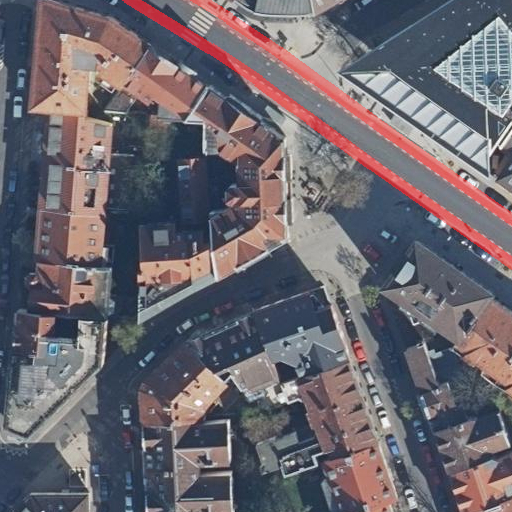
\includegraphics[width=.7\linewidth]{Bilder/cut-example.jpg} 
	\end{minipage}
	\begin{minipage}{.45\textwidth}
		\centering
		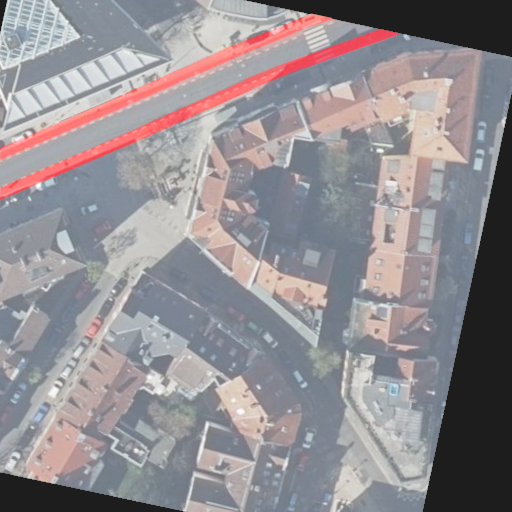
\includegraphics[width=.7\linewidth]{Bilder/augmentation-example.png} 
	\end{minipage}

	\caption{Beispielhafte Augmentierung mit Originalbild und Maske in Rot links 
	und augmentiertes (horizontale Spiegelung, Rotation, Verschiebung nach links, Helligkeit erhöht) Bild 
	mit Maske in Rot rechts.}
	\label{fig:augmentation}
\end{figure} 

% augmentation = {
% 	"rotation_range": 90,
% 	"width_shift_range": 0.1,
% 	"height_shift_range": 0.1,
% 	"fill_mode": "constant",
% 	"cval": 0,
% 	"horizontal_flip": "True",
% 	"vertical_flip": "True",
% 	"validation_split": 0.08

\section{\acf{BIoU}} \label{sec:eval:biou}

Für den Spezialfall von semantischer Segmentierung zur Erkennung von Radwegen muss für die \textit{Quality} (vgl. \autoref{sec:evaluation-metrics:quality}) 
eine Berechnungsmöglichkeit ermittelt werden, um die Quality auf diskreten Rastern, also den Bildern und Masken, anwenden zu können.
Hierfür wird der Name der \textit{\acf{BIoU}} eingeführt, der fortan für die Quality mit Anwendung auf semantische Segmentierung verwendet wird.

Sei $P$ die Prediction der Segmentierungsmaske für ein Eingabebild, $Y$ die tatsächliche Segmentierungsmaske (Ground-Truth / Label)
und $P, Y \in \{0, 1\}^{w{\times}h}$, wobei $w$ und $h$ die Breite und Höhe des Eingabebildes darstellen.
Die Einträge mit Wert eins von $P$ und $Y$ sind Radweg, die Einträge mit Wert null Hintergrund. Einträge repräsentieren Pixel.
$B$ sei die Puffergröße in Pixeln. \\
Die folgenden Formeln beziehen sich auf die Bestimmung der \ac{BIoU} \textit{einer} Prediction $P$ zu \textit{einer} Ground-Truth-Maske $Y$. 
Über einen Batch lassen sich die einzelnen \ac{BIoU}-Werte mitteln. 
Zunächst sei die Hilfsfunktion $dilate_B: \{0,1\}^{w{\times}h} \mapsto \{0,1\}^{w{\times}h}$ definiert als 
\newcommand{\norm}[1]{\left\lVert#1\right\rVert}
\begin{align}
	\label{eq:dilate} dilate_B(A) = \left( \begin{cases} 
		1 & \exists a_{kl} \in A: a_{kl} = 1 \land \norm{
			\begin{pmatrix} k \\ l \end{pmatrix} - \begin{pmatrix} i \\ j \end{pmatrix} }_2 \leq B \\
		0 & else 
	\end{cases} \right)_{1 \leq i \leq h, 1 \leq j \leq w}~.
\end{align}
Die Funktion $dilate_B$ bildet eine Matrix auf eine weitere derselben Ordnung ab, 
sodass alle Einträge gleich eins sind, die in der Eingabematrix eins sind. Zusätzlich sind alle Einträge eins, 
die im Umkreis von $B$ Pixel um eine Eins in der Eingabematrix liegen. Somit werden die positiven (Wert = 1)
Pixel der Eingabematrix um die Bufferzone erweitert.  \\
\autoref{eq:dilate_example} zeigt den Funktionswert von $dilate_B$ für eine Beispieleingabe 
bei Puffergröße $B=1$.
\begin{align}
	\label{eq:dilate_example} dilate_1\left(\begin{pmatrix} 
	0 & 0 & 1 \\ 
	0 & 1 & 0 \\ 
	0 & 0 & 0 
	\end{pmatrix}\right) = \begin{pmatrix} 
	0 & 1 & 1 \\ 
	1 & 1 & 1 \\ 
	0 & 1 & 0 
	\end{pmatrix}~.
\end{align}
Damit lassen sich die gepufferten, fehlertoleranteren wahr-positiv $tp_B$, falsch-positiv $fp_B$ und 
falsch-negativ $fn_B$ Werte berechnen: 
\begin{align}
	\label{eq:buffering} {tp}_B = \norm{dilate_{B}(Y) \odot P}_{1,1} , \\
	fn_B = \norm{Y - (Y \odot dilate_{B}(P))}_{1,1} , \\
	{fp}_B = \norm{P}_{1,1} - {tp}_B .
\end{align}
Beispielhaft und intuitiv dargestellt für $tp_B$: Es sollen auch alle Eins-Pixel als wahr-positiv aufgefasst werden,
die leicht von der Ground-Truth abweichen, also sich noch in der Pufferzone befinden. 
Hierfür wird die Pufferzone um die Ground-Truth $Y$ gelegt und das Hadamard-Produkt mit der Predicition $P$ gebildet.
Da alle Matritzen als Einträge nur 0 oder 1 enthalten, findet durch das Hadamard-Produkt eine Art Verundung statt, 
sodass im Produkt nur Einträge eins sind, die in beiden Matritzen eins sind. Der Rest ist null. 
Durch die zuvor durchgeführte Pufferung mit $dilate_B$ sind allerdings auch Einträge gleich eins, die in $Y$ 
zuvor null waren. Hierdurch besitzt das Hadamard-Produkt mehr Einträge mit eins, als bei der Berechnung der \ac{IoU}.
Diese Zahl ist genau um die Anzahl an positiven Pixeln aus $P$ größer, die in der Pufferzone liegen. 
Schließlich wird mit der $1,1$-Höldernorm für Matritzen die Anzahl an Einsen gezählt, was dann $tp_B$ ergibt. \\
Die Formel für die \ac{BIoU} pro Ausgabe ist analog zur \ac{IoU}, bis auf die Verwendung der jeweils gepufferten 
Variablen:\footnote{\autoref{code:quality} zeigt die dazugehörige Python-Implementation.}
\begin{align}
	\label{eq:quality} BIoU = \frac{tp_B}{tp_B + fp_B + fn_B} ~.
\end{align}
Für einen \ac{BIoU}-Wert über einen Batch können die individuellen Werte pro Ausgabe gemittelt werden.

\begin{figure}
	\centering
	\begin{subfigure}{.32\textwidth}
		\centering
		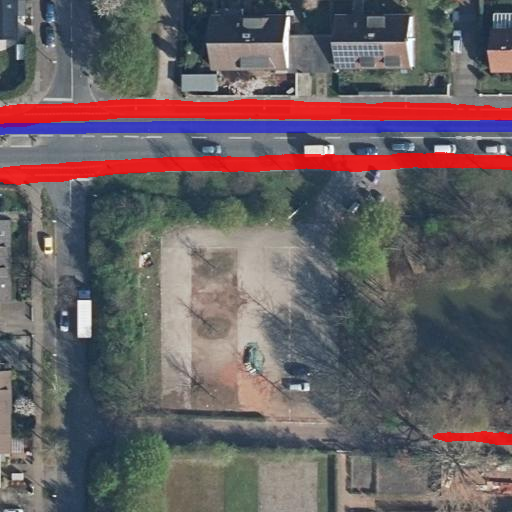
\includegraphics[width=1.\linewidth]{Bilder/biou/badish-q3918-iou0063-idx498.png}
		\caption{\ac{BIoU}: 39,18 \ac{IoU}: 0,63}
	\end{subfigure}
	\begin{subfigure}{.32\textwidth}
		\centering
		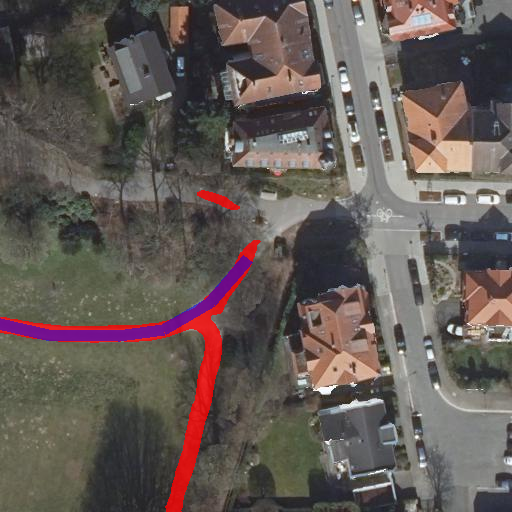
\includegraphics[width=1.\linewidth]{Bilder/biou/medium-q5804-iou3622-idx907.png}
		\caption{\ac{BIoU}: 58,04 \ac{IoU}: 36,22}
	\end{subfigure} 
	\begin{subfigure}{.32\textwidth}
		\centering
		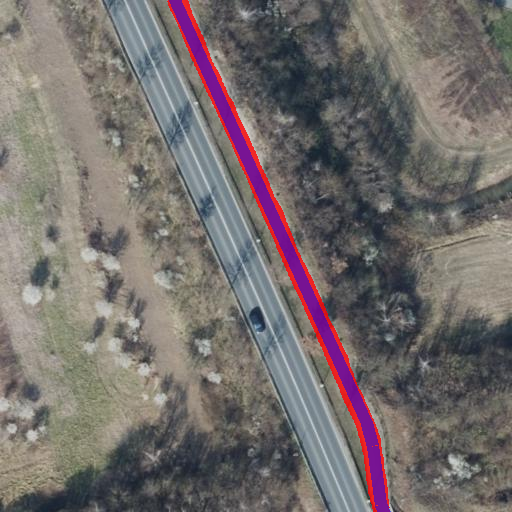
\includegraphics[width=1.\linewidth]{Bilder/biou/best-q1-iou6156-idx903.png}
		\caption{\ac{BIoU}: 100 \ac{IoU}: 61,56}
	\end{subfigure}

	\caption{Ausschnitte aus dem BikeSat-Datensatz mit roter Prediction- und blauer Ground-Truth-Maske. 
	Dazu die jeweiligen Werte für \ac{BIoU} und \ac{IoU} in Prozent.}
	\label{fig:biou-showcase}
\end{figure}

Die \ac{BIoU} adressiert das Verschiebungs-Problem der \ac{IoU} mit einem Puffer zur relaxierteren Ermittlung der 
$tp$, $fp$ und $fn$. Hierbei ist allerdings die Puffergröße in Pixeln eine wichtige Stellschraube.  
Da ein Radweg im Mittel ca. 11,8 Pixel und eine Straßenfahrbahn ca. 17,6 Pixel breit ist (s. \autoref{sec:bike-data}), 
wird der Buffer als ganze Zahl auf das arithmetische Mittel $\frac{11,8 + 17,6}{2} = 14,7 \approx 15$ festgelegt. 
Dies erlaubt eine Verschiebung des Radwegs um eine volle Breite zzgl. einer Toleranz für die leicht variierende Radwegbreite, 
nicht aber um die Breite einer Straßenfahrbahn. Hiermit soll ein realistisches Bild der Performanz des Netzes 
bezgülich der qualitativen Erkennung der Radwege gezeichnet werden und wird ergänzend zur \ac{IoU}-Metrik 
als Bewertungsfunktion eingesetzt. \\
Als Verlustfunktion ist die \ac{BIoU} allerdings ungeeignet, da wie bei der \ac{IoU} die wahr-positiven $tp$ nicht 
stärker gewichtet werden, sodass das Netz nicht bevorzugt die wahr-positiven lernt. Des Weiteren ist die \ac{BIoU} aufgrund der 
in \autoref{eq:dilate} beschriebenen Dilate-Funktion nicht bekannt differenzierbar, was für die Verlustfunktion nötig ist. 
Gegebenenfalls kann eine Ableitung für die \ac{BIoU} gefunden werden, 
die Untersuchung dessen geht allerdings über den Umfang dieser Arbeit hinaus. 
Zuletzt wird das Verwenden der \ac{BIoU} als Loss-Funktion - unter der Prämisse, dass dies möglich ist - einen weiteren 
Hyperparameter - die Puffergröße - einführen, was weiter die Komplexität des Modells erhöht.  

\autoref{fig:biou-showcase} zeigt anhand von drei Beispielen, wie die BIoU ausfällt. Hierfür wird 
der Buffer von den oben genannten 15 Pixeln genutzt. 
Die blaue Maske ist die Ground-Truth und die rote die Prediction. In (a) ist kaum 
tatsächliche Überschneidung, was sich in der IoU wiederspiegelt (0,63\%), es kann allerdings trotzdem 
klar erkannt werden, auf welcher Straßenseite sich der obere rote Radweg befindet. Die BIoU 
bestätigt diese menschliche Intuition mit einem Wert von 39,18\%. In (c) wird der Radweg perfekt getroffen
(BIoU = 100\&), die IoU beträgt allerdings nur 61,56\%, was in der Auswertung die tatsächliche Performanz 
sehr verzerrt. Zusammenfassend ist die BIoU ein Maß, das geeigneter die menschliche Intuition vertritt.

\section{Architektur} \label{sec:architecture}

Im Folgenden werden die untersuchten Architekturen genauer beschrieben und ebenfalls begründet, 
warum die jeweiligen architektonischen Entscheidungen getroffen wurden, bzw. warum bestimmte Netze verwendet werden. \\
In \autoref{sec:state-of-the-art-roads} wird ausführlich der Stand der Technik und Wissenschaft 
im Bereich der Straßenerkennung und -extraktion mittels Computer-Vision-Modellen beschrieben. 
Aufgrund der Ähnlichkeit der Problemdomäne (vgl. \autoref{sec:motivation} u. \autoref{sec:novelty}) 
lässt sich vermuten, dass ähnliche Verfahren wie 
zum Erkennen von Straßen auch für das Erkennen von Fahrradwegen nützlich sein können. 
\\
Die Radwege sollen, wie Straßen auch (s. \autoref{sec:state-of-the-art-roads}), 
mittels Image-Semantic-Segmentation von einem Computer-Vision-Modell 
markiert werden. Andere Klassifizierungsarten, wie die in \autoref{sec:aufgabenkategorien} beschriebene 
Objektdetektion würde zu grobe Bounding-Boxes um schräg verlaufende Radwege legen, sodass im Prinzip 
eine Straße markiert werden würde, die zwar einen Radweg hat, aber nicht klar wäre, wo dieser verläuft, 
bzw. ob ein Radweg in beide Richtungen existiert. Aus demselben Grund ergibt eine reine Klassifikation, 
ob ein Bild einen Radweg enthält oder nicht ebenfalls keinen Sinn. 
Auf der anderen Seite würde Instanz-Segmentierung keine weiteren relevanten Informationen hinzufügen, 
wonach semantische Segmentierung ausreicht, um das Problem zu lösen. \\
Wie bereits in \autoref{sec:state-of-the-art-roads} dargelegt, sind alle relevanten Modelle zur 
Straßenerkennung über \ac{ML} basierend auf der U-Net-Archtiektur (vgl. \ref{sec:architekturkomponenten:unet}).
Folglich sollen die hier betrachteten Modelle ebenfalls als angepasste U-Nets entworfen werden. 
Insbesondere ermöglicht dies auch die Modelle zur Fahrradwegerkennung auf den verschiedenen 
in \autoref{sec:road-detection:roads-data} vorgestellten Datensätzen zur Straßenerkennung vorzutrainieren, 
was zu allgemein besseren Ergebnissen führen kann (s. \autoref{sec:transfer-learning}). 
Außerdem können so die erzielten Ergebnisse vom Pre-Training mit den öffentlichen Benchmarks verglichen werden,
um deren Ergebnisse zu validieren und früh Fehler in den eigenen Entscheidungen und Implementationen zu entdecken.

\renewcommand{\labelenumii}{\theenumii}
\renewcommand{\theenumii}{\theenumi.\arabic{enumii}.}

Zunächst soll so ein nur leicht modifiziertes U-Net, welches im Folgenden \textit{\acf{BUNet}} 
genannt wird, entworfen werden, welches als Baseline- und Vergleichs-Netz dienen soll und 
wovon es zwei Komplexitätsvarianten, das \ac{BUNet2} mit 2 Mio. Parametern und das \ac{BUNet15} 
mit 15 Mio. Parametern geben soll. \\
Dann soll eine zweite Klasse an U-Nets beschrieben werden, die verschiedene vortrainierte \acp{CNN} (s. \autoref{sec:pretrained-backbones}) 
als Backbones für ein U-Net verwendet, da \autoref{sec:state-of-the-art-roads} gezeigt hat, 
dass im Falle der Straßendetektion die Performanz eines Netzes stark verbessert werden kann, 
indem auf Techniken und Methoden von Modellen aus anderen Teilgebieten der Computer-Vision 
zurückgegriffen wird. 
Gegebenenfalls ist das auch für die Radwegerkennung möglich. Dazu sollen mehrere Backbones untersucht werden, 
da die gewählten Backbones jeweils gut für die Straßenerkennung funktionieren und sich 
herausstellen soll, ob es einen besonders guten Backbone für die Radwegerkennung gibt. 
Folgende Liste zeigt eine Übersicht über die Netze, während die nachfolgenden Abschnitte genauer
erläutern und begründen, warum ein Backbone gewählt wurde: 
\begin{enumerate}
	\item \textit{\acf{BUNet}}: Baseline-Netz ohne Backbone.
	\begin{enumerate}
		\item \textit{\acf{BUNet2}}: Variante mit 2 Mio. Parameter.
		\item \textit{\acf{BUNet15}}: Variante mit 15 Mio. Parameter.
	\end{enumerate}
	\item Backbone-U-Nets
	\begin{enumerate}
		\item \textit{\acf{VBUNet}}: Baseline-Netz mit Baseline-Backbone.
		\item \textit{\acf{RBUNet}}: Hoch-performant bei Straßenerkennung.
		\item \textit{\acf{DBUNet}}: Hoch-performant bei Straßenerkennung.
	\end{enumerate}
\end{enumerate} 

\subsection{Bike-U-Net} \label{sec:architecture:bike-u-net}

\autoref{fig:bike-unet-2} zeigt die verwendete Architektur für das \textit{\ac{BUNet2}}. 
Hierfür wurde das in \autoref{fig:u-net-architecture} 
dargestellte originale U-Net auf den vorliegenden Anwendungsfall angepasst.
Diese Anpassungen sind in der nachfolgenden Liste \textit{begründet}. Dabei wird die Architektur auf einer 
hohen Flughöhe \textit{erläutert}. 
Eine genaue \textit{Beschreibung} der Architektur in ihrer konkreten Umsetzung 
ist im Implementationskapitel \autoref{sec:arch-impl:bunet} zu finden.  

\begin{itemize}
	\item Der Output verwendet keine explizite One-Hot-Kodierung für Fahrradweg und Hintergrund, 
	sondern eine mit lediglich einem Output-Neuron, wobei keine Aktivierung einen Hintergrundpixel 
	und eine Aktivieriung ein Radweg-Pixel impliziert, wie in \autoref{sec:state-of-the-art-roads} beschrieben, 
	um eine intuitivere Bewertung zu ermöglichen. 
	\item Im Gegensatz zum originalen U-Net (vgl. \autoref{sec:architekturkomponenten:unet}) soll der 
	Output dieselbe Bild-Dimension erhalten, wie der Input, um die Lokalisierung der semantischen Segmentierung zu verbessern.
	Das ist auch bei in \autoref{sec:state-of-the-art-roads} beschriebenen Netzen gewöhnlich und bewährt.
	\item 
	Das Bike-U-Net-2 soll eher geringere parametrische Komplexität aufweisen. 
	Die Zahl an Parametern ist somit weitaus geringer als im Original-U-Net (vgl. \autoref{sec:architekturkomponenten:unet}) angesetzt. 
	Hiermit soll getestet werden, ob auch ein recheneffizienteres und kleineres U-Net gute Ergebnisse liefert, 
	und damit weniger Regularisierung notwendig ist. \\
	Da aber die in \autoref{sec:state-of-the-art-roads} beschriebenen Netze 15-25 Mio. Parameter haben, 
	soll ein weiteres U-Net mit mehr Parametern getestet werden. Das \textit{\ac{BUNet15}} hat somit ebenfalls circa 15 Mio. 
	Parameter\footnote{\autoref{fig:bike-unet-15} zeigt \ac{BUNet15}}.
	Bis auf die parametrische Komplexität sind \ac{BUNet2} und \ac{BUNet15} identisch.
	\item Die Normalisierung und Standardisierung soll automatisch durch das Netz erfolgen. 
	Dies hat mehrere Gründe: Zum einen übernimmt so das Netz selbst die Normalisierung und Standardisierung der Daten, 
	wodurch sich das beim Vorverarbeiten gespart werden kann und zum anderen kann von den in \autoref{sec:architekturkomponenten:batchnorm} 
	beschriebenen Vorteilen, wie schnellerem Training profitiert werden, 
	ohne, dass dafür zusätzlicher Aufwand betrieben werden muss und keine Nachteile entstehen.
	\item Über Dropout (vgl. \autoref{sec:architekturkomponenten:dropout}) ist eine Regularisierung möglich. Dropout soll als 
    Hyperparameter eingebaut werden, um einfach kontrollierbar Regularisierung anzuwenden, 
	falls die Modelle Probleme mit Overfitting durch zu hohe Komplexität bekommen. 
	Aufgrund der eher wenigen Parameter wird dies aber gegebenenfalls nur beim \ac{BUNet15}, 
	oder überhaupt nicht, nötig.
	\item Die Aktivierungsfunktion trägt zu der Lernfähigkeit des Netzes bei (Robustheit gegen das Vanishing-Gradient-Problem), 
	es sind alle Netzteile möglichst beteiligt, um die Komplexität zu nutzen (Resistenz gegen das Dying-Neuron-Problem) und
	numerisch zu große Aktivieriungen sind vermieden. 
	\item Für das Ouptut-Layer soll eine probabilistische Aktivierungsfunktion verwendet werden, 
	um die Ergebnisse leichter zu interpretieren.
\end{itemize}

\begin{figure}
	\centering
	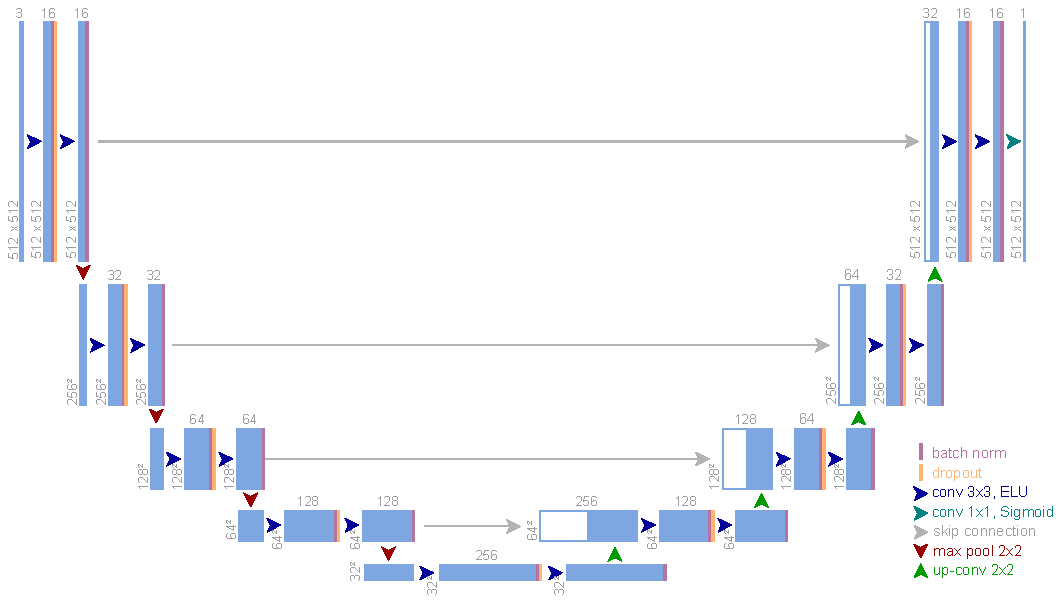
\includegraphics[width=1.\textwidth]{Bilder/own-unet-2mil.pdf} 
	\caption{Bike-U-Net-2 mit 1,946 Mio. Parametern.}
	\label{fig:bike-unet-2}
\end{figure} 

% HE INITIALIZATION

\subsection{Backbone-U-Nets}

Dieser Abschnitt beschreibt, warum die Backbone-U-Nets, wie in \autoref{sec:pretrained-as-unet-backbone} beschrieben gebildet,
für diese Arbeit relevant sind und untersucht werden. Wie diese konkret in ihrer Architektur umgesetzt sind, 
wird im Implementationskapitel \autoref{sec:arch-impl} detailliert.  

\subsubsection{VGG16-Bike-U-Net}

\textit{\ac{VBUNet}} nutzt das in \autoref{sec:pretrained-backbones:vgg16} beschriebene Netz VGG16 
mit auf ImageNet vortrainierten Gewichten als Backbone. 
VGG16 wird als Backbone ausgewählt und getestet, da es als eine Art Basis- bzw. Standardversion der nachfolgenden 
Backbone-Netze aufgefasst werden kann, da diese auf VGG16 aufbauen und dieses - zumindest 
für den ImageNet-Datensatz - verbessern und nachvollzogen werden soll, ob diese Anpassungen dienlich sind 
für den konkreten Anwendungsfall der Radwegerkennung. Zudem ist VGG16 sehr beliebt als vortrainiertes 
Netz, weswegen es viele Vergleichsmöglichkeiten gibt. 
Des Weiteren wird VGG16 als Backbone in Research zum Pre-Training mit U-Nets eingesetzt (s. \autoref{sec:transfer-learning:backbones}), 
auf dessen Ergebnisse diese Arbeit aufbaut. 
Demnach ist es wiederum für Vergleichszwecke sinnvoll VGG16 als Backbone für die Radwegerkennung zu verwenden.   

\subsubsection{ResNet34-Bike-U-Net}

\textit{\ac{RBUNet}} nutzt das in \autoref{sec:pretrained-backbones:resnet} beschriebene Netz ResNet34 
mit auf ImageNet vortrainierten Gewichten als Backbone. 
ResNet34 wird als Backbone ausgewählt und getestet, aufgrund der hohen Präsenz von 
Residual-Blöcken in den leistungsstärksten Modellen 
zur Straßenerkennung aus \autoref{sec:state-of-the-art-roads} und insbesondere \autoref{tab:optimized-benchmarks}.
Es wird sich ebenfalls eine bessere Performanz dieses Modells bei der Radwegerkennung erhofft. 

\subsubsection{DenseNet121-Bike-U-Net}

\textit{\ac{DBUNet}} nutzt das in \autoref{sec:pretrained-backbones:densenet121} beschriebene Netz DenseNet121 
mit auf ImageNet vortrainierten Gewichten als Backbone.
DenseNet121 wird als Backbone ausgewählt, wegen der guten Ergebnisse von Dense-U-Net-121 aus \autoref{sec:state-of-the-art-roads}. 
Darüber hinaus werden zusammen mit VGG16 und ResNet34 Netze mit verhältnismäßig flacher, mitteltiefer und tiefer 
Architektur getestet, was eine Vielfalt an Architekturen abbildet.

\section{Hyperparameter} \label{sec:hyperparameter}

\subsubsection{Batch-Size:}

Der Vorteil einer kleineren Batch-Size ist, dass das Netz besser lernt die Feinheiten der Daten abzubilden. 
Der Vorteil einer görßeren Batch-Size ist, dass das Netz schneller trainiert. 
Da allerdings Batch-Norm (vgl. \autoref{sec:architecture}) angewandt wird, würde eine Batch-Size von 1 (wie im originellen U-Net) keinen 
Sinn ergeben, da die Daten im Pre-Processing nicht normalisiert werden (vgl. \autoref{sec:pre-processing}), wodurch Batch-Norm alle 
Normalisierung übernimmt. Wenn das allerdings auf nur ein Bild angewandt wird, ist keine gute Normalisierung über den ganzen Datensatz zu erwarten. 
Eine große Batch-Size, wie z.B. 16, ist allerdings sehr ressourcenintensiv, da alle Elemente des Batches simultan in den Speicher geladen und verarbeitet 
werden müssen. \\
Als Kompromiss wird eine Batch Size von 4 festgehalten. Durch die zufälligen Batches ist eine angemessene Normalisierung zu erwarten.

\subsubsection{Dropout-Rate:} \label{sec:hyperparameter:dropout}

Dropout soll dem Overfitting, was aufgrund der wenigen Trainingsdaten auftreten kann, entgegen wirken. 
Die Rate, mit der die Dropout-Layer Neuronen auf null setzen, wird nicht als ein konstanter Wert für das ganze Netz festgelegt, 
sondern nimmt im Encoder-Teil sukzessive zu und ab dem Decoder-Teil gespiegelt sukzessive ab, siehe \autoref{tab:dropout}. 
Das soll eine hohe Dropout-Rate im Mittelteil des Netzes ermöglichen, während die Rate in den äußeren Schichten eher niedrig ist. 
Dies ist erwünscht, damit in den äußeren Schichten, möglichst alle Inputs eingefangen werden bzw. die Outputs richtig lokalisiert werden. 
In den äußeren Schichten mit eher weniger Filtern und damit weniger Parametern stellt Overfitting ein geringeres Problem dar. 
Für die mittleren Layer mit ausgeprägten Feature-Maps, vielen Filtern und Parametern jedoch ein größeres Problem, weswegen hier ein eher größerer
Dropout erwünscht ist.     

\begin{table}[ht]
	\centering
	\begin{tabular}{r|ll|ll|l|ll|ll}
		\textbf{Block} & 1 & 2 & 3 & 4 & 5  & 6 & 7 & 8 & 9 \\
		\midrule
		\textbf{Rate} & 0,1 & 0,1 & 0,2 & 0,2 & 0,3 & 0,2 & 0,2 & 0,1 & 0,1 \\ 
	\end{tabular}
	\caption{Dropout-Raten der unterschiedlichen Blöcke in \ac{BUNet}.}
	\label{tab:dropout}
\end{table}

\subsubsection{Learning-Rate:}

Als Learning-Rate wird ein Faktor von $0,0001$ angesetzt. Dieser Wert wird in einigen verwandten Problemen mit U-Nets genutzt, 
weswegen der Wert auch hier zu Beginn verwendet wird. Falls das Training damit sehr langsam ist oder nicht konvergiert, 
kann der Wert angepasst werden. Durch einen Scheduler wird während des Trainings die Learning-Rate bei stagnierendem Fortschritt 
herabgesetzt, was in \autoref{sec:training} genauer erläutert ist. 

\section{Pre-Training auf Straßendatensätzen} \label{sec:pre-training-roads}

Für das Pre-Training auf Straßendatensätzen werden die Datensätze \textit{DeepGlobe} und \textit{Massachusetts} 
(vgl. \autoref{sec:road-detection:roads-data}) zu dem \textit{Combined}-Datensatz zusammengefasst. 
Dabei sind die Vorteile eines heterogenen Pre-Trainings genutzt: Es sind sowohl homogene amerikanische Städte (Massachusetts), 
als auch sehr heterogene weltweite städtische und ländliche Straßen (DeepGlobe) enthalten, wodurch 
die grundlegenden Features, die Straßen ausmachen, sehr generalisiert gelernt werden sollen. Damit lassen sich diese 
Features auf die Radwegerkennung übertragen. Zudem wurden diese beiden Datensätze gewählt, da sie die größten öffentlich zugänglichen 
im Gebiet der Straßenerkennung darstellen und die viele der in diesem Kapitel vorgenommenen Entscheidungen 
auf den Ergebnissen zu diesen Datensätzen basieren, sowie eine hohe Vergleichbarkeit möglich ist. 
Auf weitere Datensätze wird verzichtet, da der Combined-Datensatz mit 25294 $512{\times}512$-Ausschnitten 
bereits eine angemessene Größe hat und weitere Datensätze die Bewertung des Pre-Trainings erschweren und Vergleichswerte 
darauf nicht zugänglich sind. 

Der DeepGlobe-Datensatz kann ohne weiteres übernommen werden und nach den Regeln in \autoref{sec:pre-processing} vorverarbeitet werden. \\ 
Für den Massachusetts-Datensatz wird eine weitere Vorverarbeitung vorgenommen. Der Massachusetts-Datensatz 
besteht aus einem Ausschnitt von Massachusetts in Form eines unregelmäßigen Polygon. Viele der $512{\times}512$-Zuschnitte enthalten 
also große, weiße Flächen ohne Bild. Der BikeSat-Datensatz enthält ebenfalls Zuschnitte mit schwarzen Flächen, 
doch im Gegensatz zum BikeSat-Datensatz hat der Massachusetts-Datensatz das Problem, dass die Masken nicht von einem 
unregelmäßigen Massachusetts-Ausschnitt genommen sind, sondern von einem quadratischen, sodass in den weißen Flächen 
der Bilder in der dazugehörigen Maske an dießen Stellen Straßen eingezeichnet sind, wie \autoref{fig:problem-mass} illustriert. 
Dadurch sieht das Netz also willkürlich 
im weißen (RGB = (255, 255, 255)) Bereich als Straßen annotierte weiße Pixel. Um diese Verwirrung aufzulösen, werden 
für den Combined-Datensatz alle Bild-Ausschnitte mit über 10\% weißer Fläche entfernt. 
Ansonsten unterliegt es dem gleichen Pre-Processing wie die sonstigen Datensätze (vgl. \autoref{sec:pre-processing}). 

Schließlich werden beide Datensätze gemischt und in einen Training-Validation-Test-Split unterteilt und diese Splits werden zum 
Combined-Datensatz vereinigt, wofür der Split in \autoref{tab:combined-split} abgebildet ist. 
Die Datensätze werden vor dem Zusammenfügen aufgespalten, damit das relative Verhältnis in allen Teildatensätzen gleich ist.  

\begin{figure}
	\centering
	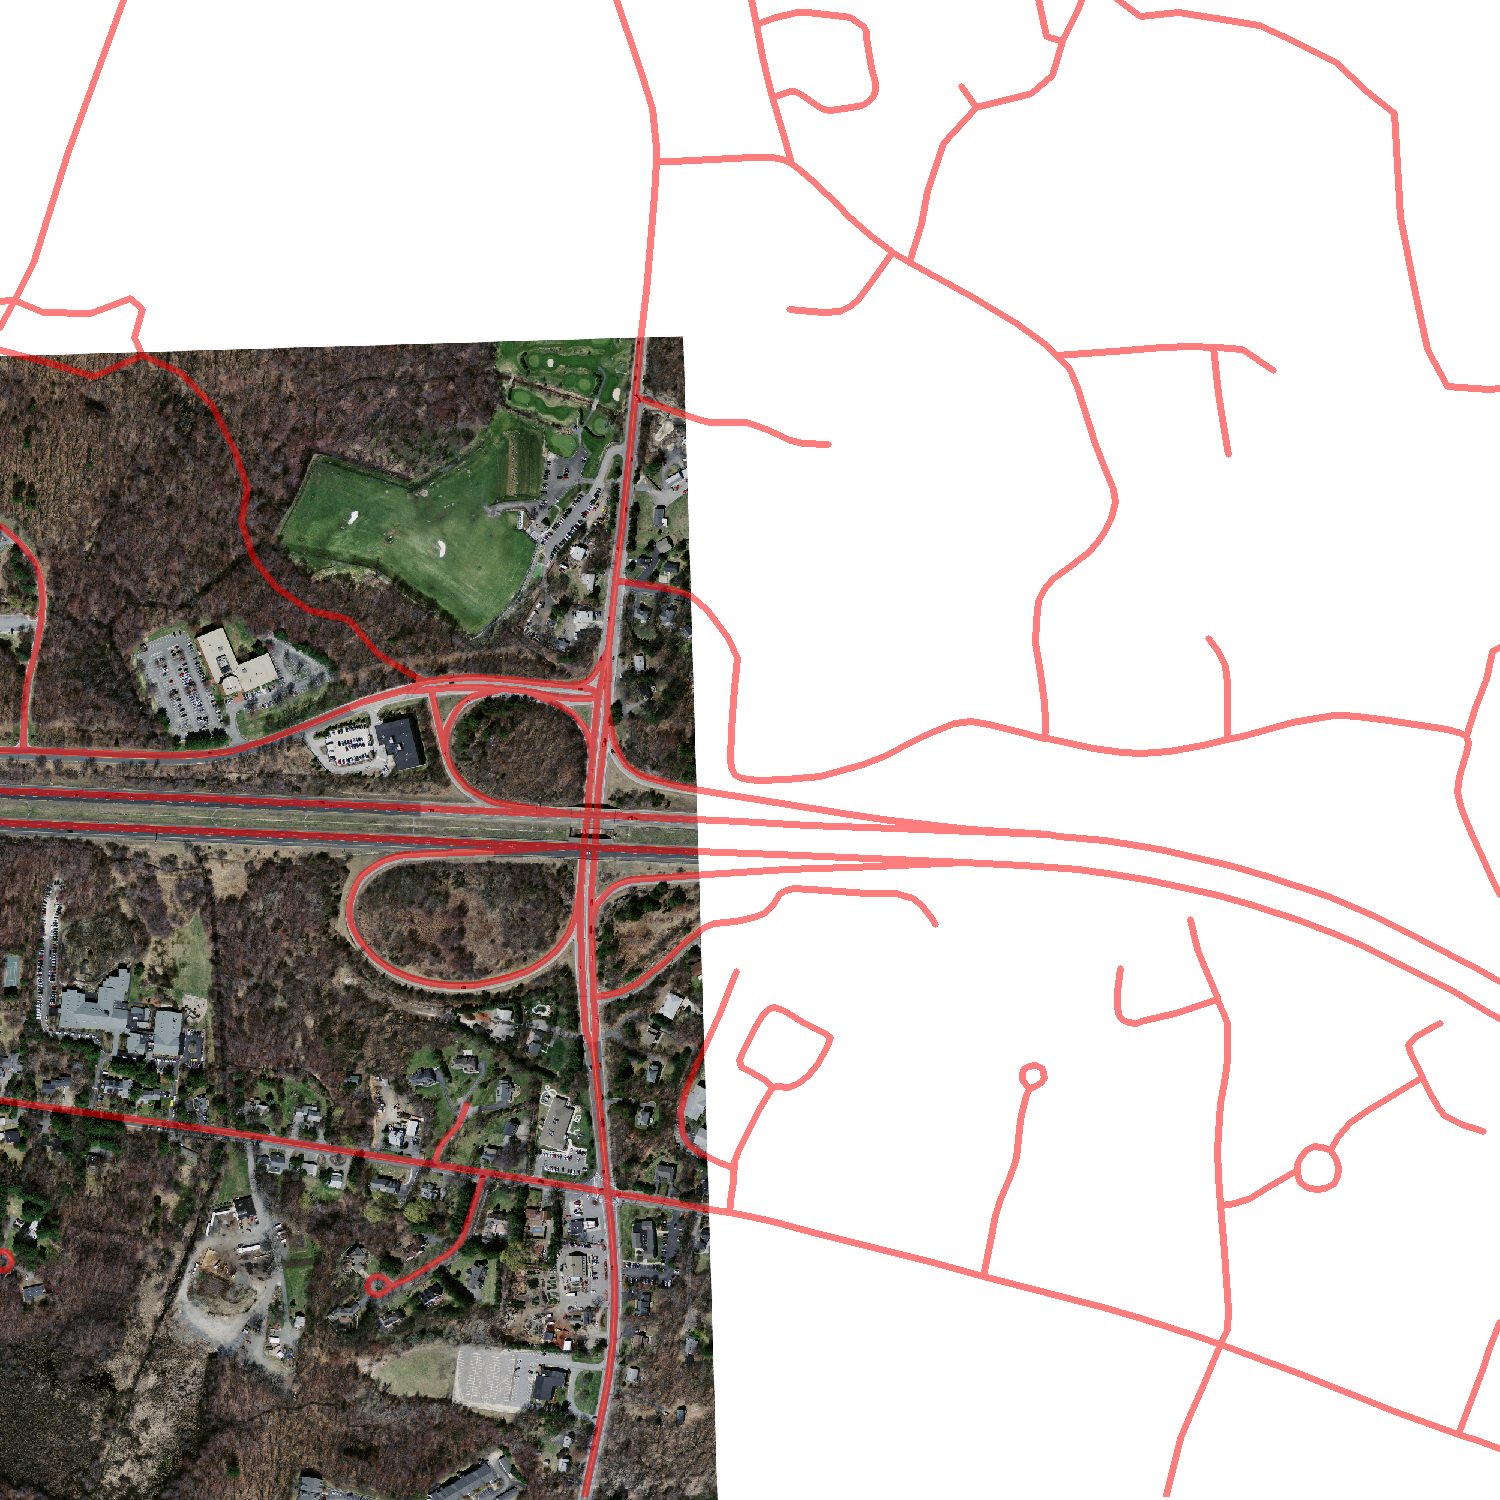
\includegraphics[width=.5\textwidth]{Bilder/problem_mass.png} 
	\caption{Beispiel des Problems im Massachusetts-Datensatz: In den Randbereichen sind Masken (rotes Overlay) in Bereichen eingezeichnet, 
	in denen kein Bild vorhanden ist.}
	\label{fig:problem-mass}
\end{figure} 

\begin{table}[ht]
	\centering
	\begin{tabular}{l|l|l|l|l}
		& Training & Val. & Test & Summe \\
		\midrule
		Absolut & 18598 & 1617 & 5079 & 25294 \\
		Anteil & 73,5 & 6,4 & 20,1 & 100 \\ 
	\end{tabular}
	\caption{Training-Validation-Test-Split des \textit{Combined}-Datensatzes, welcher aus DeepGlobe und Massachusetts besteht, 
	in gefilterten $512{\times}512$-Ausschnitten.}
	\label{tab:combined-split}
\end{table}

Nach der Erstellung des Datensatzes werden alle in \autoref{sec:architecture} vorgestellten Netze
auf dem Combined-Datensatz trainiert. 
Die \autoref{acro:BUNet}-Netze werden dabei von Grund auf neu trainiert nach den Regeln aus \autoref{sec:training}, 
wobei für die Backbone-Netze folgend Form des Fine-Tunings des Transfer-Learning angewandt wird (vgl. \autoref{sec:transfer-learning:backbones}): 
Der Encoder der Backbone-Netze ist auf ImageNet vortrainiert. Der Encoder ist für die ersten 12 Epochen des Trainings eingefroren, 
während nur der Decoder trainiert wird. Dann  wird die Learning-Rate um Faktor 10 verringert, der Encoder 
auf trainierbar gestellt und das Training fortgesetzt bis entweder 100 Epochen verstrichen sind oder das Training 
zuvor gestoppt wird, wie in \autoref{sec:training} detailliert.    

\section{Training} \label{sec:training}

Zunächst Allgemeines zum Training:
Der Validation-Datensatz wird genutzt, um nach jeder Trainingsepoche den Verlust dieses Datensatzes zu bestimmen. 
Verbessert sich der Validation-Verlust nach fünf Epochen nicht, wird die Lernrate um Faktor 10 verringert. 
Verbessert sich der Validation-Verlust nach sieben Epochen nicht, wird der beste Stand, mit der Epoche mit geringstem 
Validation-Verlust, wiederhergestellt und das Training vorzeitig beendet.  \\
Am Ende jeder Epoche wird der Trainingsdatensatz gemischt, sodass in der nächsten Epoche neue zufällige 
Batches mit neuer Augmentierung entstehen. \\
Es wird maximal 100 Epochen trainiert.

\begin{figure}[h]
	\centering
	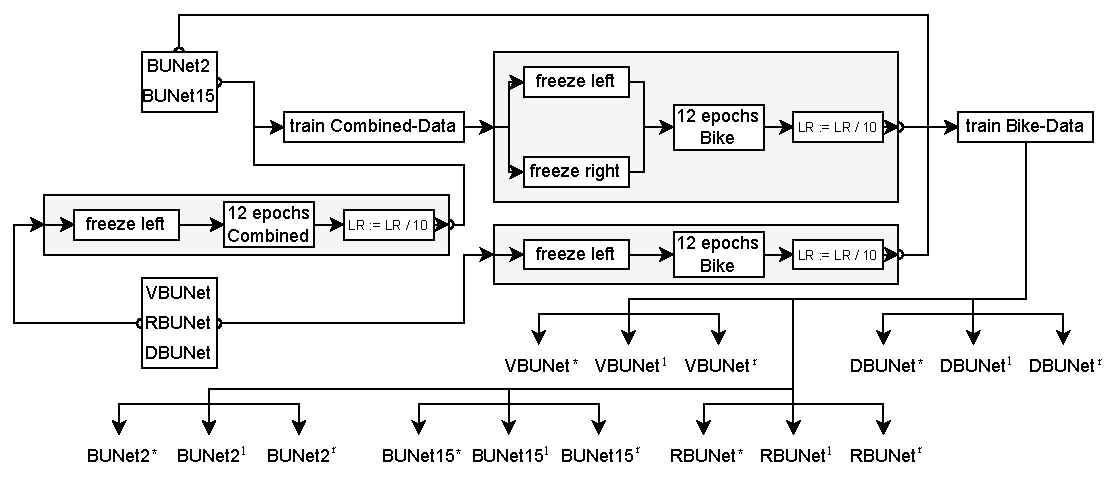
\includegraphics[width=1.\textwidth]{Bilder/training-concept.drawio.pdf} 
	\caption{Training-Konzept der Architekturen aus \autoref{sec:architecture}. * heißt kein Pre-Training,
	hochgestelltes l vortrainiert und Fine-Tuning mit eingefrorenem Encoder, hochgestelltes r Fine-Tuning mit eingefrorenem Decoder.}
	\label{fig:training}
\end{figure} 

Ziel soll es sein, die beste Architektur für das Erkennen von Radwegen zu finden und zu untersuchen,
ob es starke Unterschiede bei den verwendeten Fine-Tuning-Techniken gibt. 
\autoref{fig:training} zeigt, wie die Architekturen aus \autoref{sec:architecture} trainiert werden. 
Abzweigende Pfeile bedeuten, dass der Input dupliziert wird und beide Wege verfolgt. 
Die Architekturen sind links im Diagramm zu sehen, wobei \ac{BUNet2} und \ac{BUNet15} den \ac{BUNet}-Block 
bilden und die Backbone-Architekturen einen Block. Die \acp{BUNet} werden jeweils direkt auf 
dem BikeSat-Datensatz trainiert (Pfeil ganz oben) und jeweils direkt auf dem Combined-Datensatz aus \autoref{sec:pre-training-roads}
vortrainiert und dann diese vortrainierten \acp{BUNet} jeweils fine-tuned, indem ein mal die linke Hälfte des 
Netzes (der Encoder) und ein mal die rechte Hälfte (der Decoder) eingefroren, als nicht modifizierbar gesetzt, werden,
das Training so 12 Epochen vollzogen wird, dann die Lernrate verkleinert wird um Faktor 10 und daraufhin weiter 
das \textit{ganze} Netz trainiert wird, bis es zum vorzeitigen Ende kommt oder 100 Epochen erreicht wird. \\
Die Backbone-Netze werden, wie in \autoref{sec:pre-training-roads} beschrieben, jeweils auf dem Combined-Datensatz vortrainiert
(wobei natürlich nur die linke Hälfte, also der Encoder, eingefroren wird) und dann jeweils auf dem BikeSat-Datensatz 
fine-tuned wie die \acp{BUNet}. Die Backbone-Netze werden zusätzlich ohne Pre-Training direkt auf dem BikeSat-Datensatz 
trainiert, wobei der Ablauf derselbe ist wie für den Combined-Datensatz. \\
Es resultieren Netze, die \textit{nicht} auf dem Combined-Datensatz vortrainiert sind (hochgestellter *), 
vortrainiert und über ein linksseitiges Einfrieren fine-tuned sind (hochgestelltes l) oder vortrainiert und über ein 
rechtsseitiges Einfrieren fine-tuned sind (hochgestelltes r). 

Das Fine-Tuning über links- und rechtsseitiges Einfrieren wird genutzt, da daraus klar werden soll, ob die unterschiedlichen 
Fine-Tuning-Methoden zu einem signifikanten Unterschied in der Performanz führen, was sehr problemspezifisch ist, 
wie aus der Literatur (vgl. \autoref{sec:transfer-learning}) hervorgeht. 

Weiter werden die verschiedenen trainierten Modelle durch die Test-Partition des BikeSat-Datensatzes und durch den Karlsruhe-Datensatz 
getestet und über die in \autoref{sec:evaluation} ausgewählten Maße bewertet.


% \begin{algorithm}
% 	\caption{Algorithmus zum Propagieren und Akkumulieren von Knotenwerten.}\label{lst:prop}
% 	\begin{algorithmic}[1]
% 		\Procedure{Reduce}{$G = (V,E)$} \Comment{$\forall v \in V: value(v) = weight(type(v))$}
% 			\State $sortedNodes \gets topoSort(G)$
% 			\For{$v \in sortedNodes$}\Comment{iteration in topological order}
% 				\If{$v \in R$} 
% 					\State $succ \gets successor(v)$ \Comment{$d^+_G(v) = 1$}
% 					\State $value(succ) \gets value(succ) + value(v)$
% 				\EndIf
% 			\EndFor
% 		\EndProcedure
% 	\end{algorithmic}
% \end{algorithm}

% Nun da alle Knoten die neuen kumulierten Werte haben, lassen sich die reduzierbaren Knoten $r \in R$ entfernen. 

% \mathchardef\mhyphen="2D

% \begin{algorithm}
% 	\caption{Algorithmus zum Kopieren nötiger Kanten von reduzierten Knoten.}\label{lst:reduce}
% 	\begin{algorithmic}[1]
% 		\Procedure{Reduce}{$G = (V,E), C = (F, E_F)$} \Comment{$E_F = \emptyset$}
% 			\State $sortedNodes \gets topoSort(G)$
% 			\For{$v \in sortedNodes$}\Comment{iteration in topological order}
% 				\If{$v \in F$} 
% 					\For{$succ \in successors(v)$}\Comment{$d^+_G(v) \neq 1$}
% 						\If{$succ \in F$}
% 							\State $E_F \gets E_F \cup \{(v, succ)\}$ \Comment{copy $fork \rightarrow fork$}
% 						\EndIf
% 					\EndFor
% 				\Else \Comment{$v \in R$}
% 					\State $succ \gets successor(v)$ \Comment{$d^+_G(v) = 1$}
% 					\For{$pred \in predecessors(v)$}
% 						\If{$pred \in F \land succ \in R$}
% 							\State $E \gets E \cup \{(pred, succ)\}$\Comment{connect $fork \rightarrow non \mhyphen fork$}
% 						\ElsIf {$pred \in F \land succ \in F$}
% 							\State $E_F \gets E_F \cup \{(pred, succ)\}$ \Comment{copy $fork \rightarrow fork$}
% 						\EndIf
% 					\EndFor
% 				\EndIf
% 			\EndFor\label{euclidendwhile}
% 		\EndProcedure
% 	\end{algorithmic}
% \end{algorithm}

% \pagebreak % manueller seitenumbruch

% \section{Gänzliche Einsparung gemeinsamer Teilgraphen} \label{sec:skip_entirely}

% \begin{wrapfigure}{l}{0.35\textwidth}
% 	\centering
% 	\vspace{-30pt} % Manchmal möchte man den oberen Abstand selbst anpassen
% 	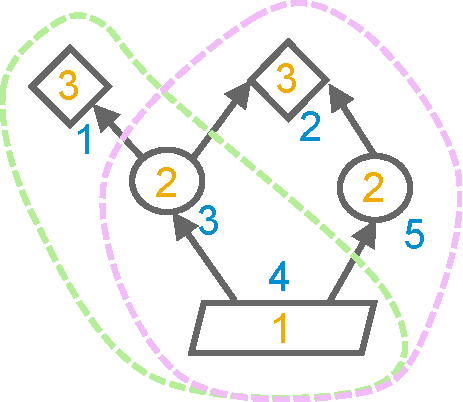
\includegraphics[width=0.30\textwidth]{Bilder/problem_illustration.pdf}
% 	\vspace{-10pt}
% 	% Das folgende ist ein Trick, um "Abbilgung x.y" in eine
% 	% eigene Zeile zu packen. Der Text zwischen [ und ] steht
% 	% im Abbildungsverzeichnis. Der Text darunter wird
% 	% tatsächlich angezeigt.
% 	\caption[Minimalbeispiel zur Teilgraph-Überspringungs-Problematik. Legende wie in \autoref{fig:trans_closures}.]{\unskip}
% 	Minimalbeispiel zur Teilgraph-Überspringungsproblematik. Legende wie in Abb. \ref{fig:trans_closures}.
% 	\label{fig:prob_illu}
% \end{wrapfigure}

% Leider lassen sich bei dem Vergleich zweier Submodelle gemeinsame Teilgraphen nicht gänzlich einsparen, indem der Similarity-Wert über Forks hinaus propagiert wird, um so jedem Knoten im Graph die Summe aller Knotenwerte unter ihm zuzuordnen, da ein gemeinsamer Teilgraph über mehrere Forks betreten werden kann (z.B. der Teilgraph der Schnittmenge von grün und lila in \autoref{fig:trans_closures} kann über Knoten 6 und 5 betreten werden) und nur der maximale Teilgraph gezählt werden darf - ansonsten würde es zu einer doppelten Wertung eines oder mehrerer Knoten kommen. Auch ist die Maximalität  des gemeinsamen Teilgraphen nur mit erheblichen Rechenaufwand, der dem Prinzip des Auslassens entgegensteht, zu überprüfen. Der Graph aus \autoref{fig:prob_illu} ist zur Veranschaulichung geeignet: Es ist schwierig Knoten 4 mit Wert 1 genau einmal zu zählen. Wird Knoten 3 betreten und der restliche Teilgraph (Knoten 4) übersprungen, so wird der Wert 3 zur Similarity addiert.
